% ven diagrams using tikz package


\documentclass{standalone}

%maths
\usepackage{tikz}
\usepackage{scalerel}
\usepackage{pict2e}
\usepackage{tkz-euclide}
\usetikzlibrary{calc}
\usetikzlibrary{patterns,arrows.meta}
\usetikzlibrary{shadows}
\usetikzlibrary{external}

%pgfplot

\usepackage{pgfplots}
\pgfplotsset{compat=newest}
\usepgfplotslibrary{statistics}
\usepgfplotslibrary{fillbetween}

%colours
\usepackage{xcolor}



\begin{document}

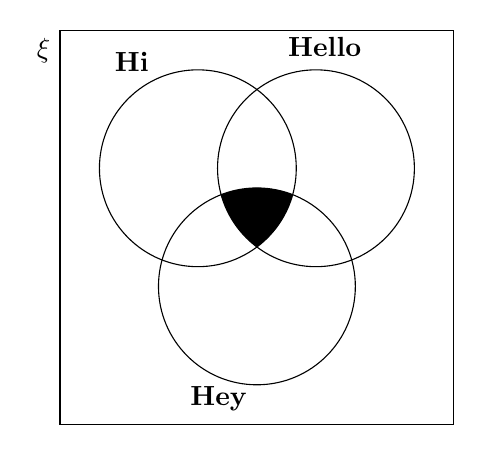
\begin{tikzpicture}


\coordinate (a) at (0,0);
\coordinate (b) at (1.5,0);
\coordinate (c) at (0.75,-1.5);

\draw (a) circle (1.25);
\draw (b) circle (1.25);
\draw (c) circle (1.25);

\draw (-1.75,-3.25) rectangle (3.25,1.75);

\coordinate [label=left:$\xi$] (R) at (-1.75, 1.5);
\coordinate [label= above left:\textbf{Hi}] (A) at (-0.5, 1.1);
\coordinate [label= above left:\textbf{Hello}] (B) at (2.2,1.3);
\coordinate [label= above left:\textbf{Hey}] (C) at (0.75,-3.2);



\clip (a) circle (1.25);
\clip (b) circle (1.25);
\clip (c) circle (1.25);

\fill (c) circle (1.25);







\end{tikzpicture}

\end{document}